\section{Methoden}

\subsection{Teststrategie}

Wie im Vorsemester im Modul \textit{Software Testing} eingeübt, sollen die \textit{Agile Test Quadrants} (\imgref{fig:agile-testing-quadrants}) als Grundlage zur Erarbeitung einer Teststrategie dienen \cite[p. XX]{agiletest}.

\begin{figure}
	\centering
	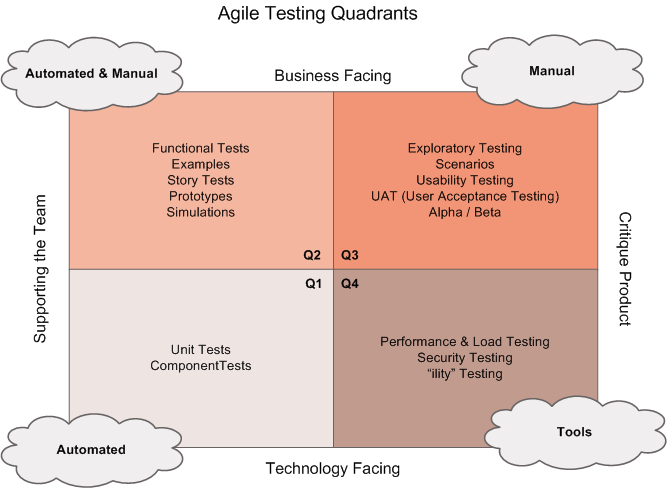
\includegraphics[width=\linewidth]{pics/agile-testing-quadrants.png}
	\caption{\textit{Agile Testing Quadrants} nach Lisa Crispin (\url{https://lisacrispin.com/2011/11/08/using-the-agile-testing-quadrants/})}
	\label{fig:agile-testing-quadrants}
\end{figure}
